\documentclass[border=5pt]{standalone}
\usepackage[utf8]{inputenc}
\usepackage[T1]{fontenc}
\usepackage{tikz}
\usepackage{pgfplots}
\pgfplotsset{compat=1.18}

\definecolor{stresslow}{RGB}{76,175,80}
\definecolor{stressmed}{RGB}{255,193,7}
\definecolor{stresshigh}{RGB}{244,67,54}

\begin{document}
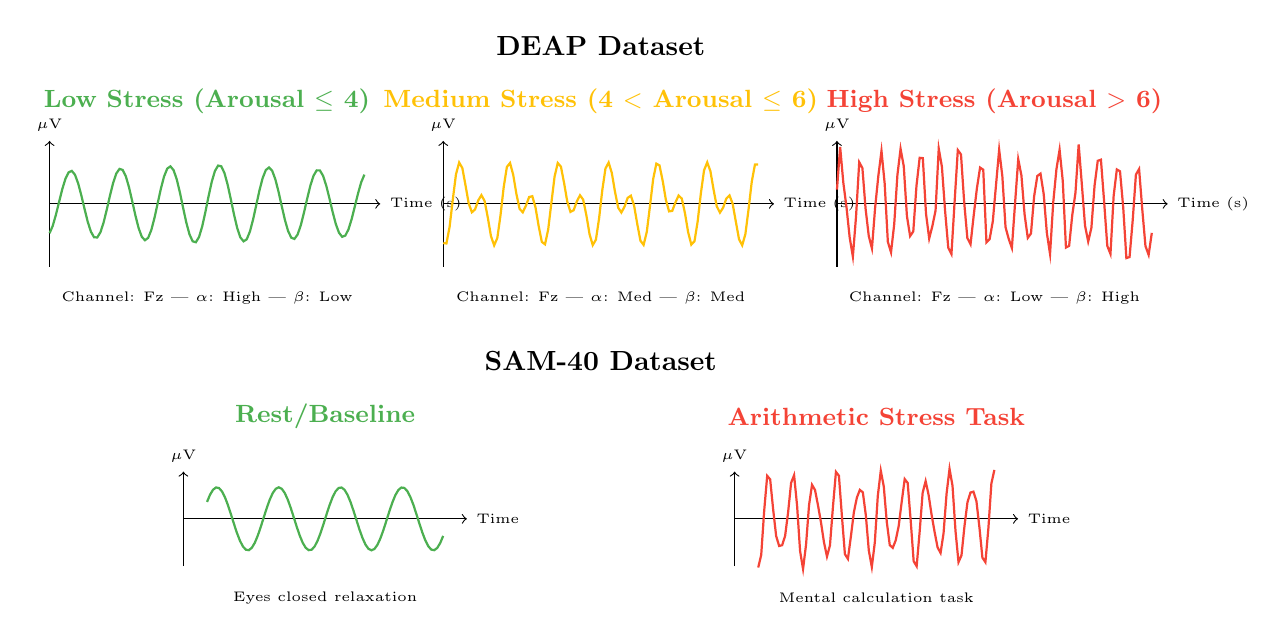
\begin{tikzpicture}
% DEAP Dataset Examples
\node[font=\bfseries] at (0,4.5) {DEAP Dataset};

% Low Stress - DEAP
\node[font=\small\bfseries, text=stresslow] at (-5,3.8) {Low Stress (Arousal $\leq$ 4)};
\begin{scope}[shift={(-5,2.5)}]
\draw[->] (-2,0) -- (2.2,0) node[right, font=\tiny] {Time (s)};
\draw[->] (-2,-0.8) -- (-2,0.8) node[above, font=\tiny] {$\mu$V};
% Alpha-dominant relaxed signal
\draw[stresslow, thick] plot[domain=-2:2, samples=100] (\x, {0.5*sin(10*\x r)*exp(-0.1*abs(\x))});
\node[font=\tiny] at (0,-1.2) {Channel: Fz | $\alpha$: High | $\beta$: Low};
\end{scope}

% Medium Stress - DEAP
\node[font=\small\bfseries, text=stressmed] at (0,3.8) {Medium Stress (4 $<$ Arousal $\leq$ 6)};
\begin{scope}[shift={(0,2.5)}]
\draw[->] (-2,0) -- (2.2,0) node[right, font=\tiny] {Time (s)};
\draw[->] (-2,-0.8) -- (-2,0.8) node[above, font=\tiny] {$\mu$V};
% Mixed frequency signal
\draw[stressmed, thick] plot[domain=-2:2, samples=100] (\x, {0.3*sin(10*\x r) + 0.3*sin(20*\x r)});
\node[font=\tiny] at (0,-1.2) {Channel: Fz | $\alpha$: Med | $\beta$: Med};
\end{scope}

% High Stress - DEAP
\node[font=\small\bfseries, text=stresshigh] at (5,3.8) {High Stress (Arousal $>$ 6)};
\begin{scope}[shift={(5,2.5)}]
\draw[->] (-2,0) -- (2.2,0) node[right, font=\tiny] {Time (s)};
\draw[->] (-2,-0.8) -- (-2,0.8) node[above, font=\tiny] {$\mu$V};
% Beta-dominant stressed signal
\draw[stresshigh, thick] plot[domain=-2:2, samples=100] (\x, {0.6*sin(25*\x r) + 0.2*rand});
\node[font=\tiny] at (0,-1.2) {Channel: Fz | $\alpha$: Low | $\beta$: High};
\end{scope}

% SAM-40 Dataset Examples
\node[font=\bfseries] at (0,0.5) {SAM-40 Dataset};

% Rest/Baseline - SAM40
\node[font=\small\bfseries, text=stresslow] at (-3.5,-0.2) {Rest/Baseline};
\begin{scope}[shift={(-3.5,-1.5)}]
\draw[->] (-1.8,0) -- (1.8,0) node[right, font=\tiny] {Time};
\draw[->] (-1.8,-0.6) -- (-1.8,0.6) node[above, font=\tiny] {$\mu$V};
\draw[stresslow, thick] plot[domain=-1.5:1.5, samples=80] (\x, {0.4*sin(8*\x r)});
\node[font=\tiny] at (0,-1) {Eyes closed relaxation};
\end{scope}

% Stress Task - SAM40
\node[font=\small\bfseries, text=stresshigh] at (3.5,-0.2) {Arithmetic Stress Task};
\begin{scope}[shift={(3.5,-1.5)}]
\draw[->] (-1.8,0) -- (1.8,0) node[right, font=\tiny] {Time};
\draw[->] (-1.8,-0.6) -- (-1.8,0.6) node[above, font=\tiny] {$\mu$V};
\draw[stresshigh, thick] plot[domain=-1.5:1.5, samples=80] (\x, {0.5*sin(22*\x r) + 0.15*sin(35*\x r)});
\node[font=\tiny] at (0,-1) {Mental calculation task};
\end{scope}
\end{tikzpicture}
\end{document}
